\chapter{Benchmarking}


\section{Traccia}
 Si comparino due sistemi con lo stesso sistema operativo e processori diversi usando il benchmark \textit{N-Body}, il quale simula l'evoluzione di un sistema di n corpi sotto l'influenza della forza di gravità.
 Il simulatore N-body è un buon benchmark poichè stressa:

\begin{itemize}
    \item L'unità di calcolo in virgola mobile (Floating-point unit);
    \item Il meccanismo di gestione dello Stack tramite chiamate ricorsive;
\end{itemize}

\section{Descrizione dell'esperimento}
Le caratteristiche dei due sistemi, \textit{A} e \textit{B}, sono riportate in \cref{tab:bench_specs}.

\begin{table}
\centering
    \begin{tabular}{|l|p{0.3\linewidth}|p{0.3\linewidth} |}
    \hline
    \multicolumn{1}{|c|}{\textbf{Caratteristiche}} &
    \multicolumn{1}{c|}{\textbf{Sistema A}} & 
    \multicolumn{1}{c|}{\textbf{Sistema B}}  \tabularnewline \hline

CPU & AMD Ryzen 7, 3700X 3.6 GHz, L3 32MB & AMD Ryzen 7, 4500U 2.0GHz, L3 8MB \tabularnewline \hline

RAM & DDR4 16GB, 3200 MHz & DDR4 SODIMM 16GB, 3200 MHz \tabularnewline \hline

OS & Windows 10 & Windows 11 \tabularnewline \hline
\end{tabular}
\caption{Tabella riassuntiva delle caratteristiche dei due sistemi a cui è stato sottoposto il benchmark}
\label{tab:bench_specs}
\end{table}

Per entrambi i sistemi, sono stati raccolti $10$ pre-campioni indipendenti (ottenuti attraverso un riavvio della macchina) simulando un milione di corpi per $30$ ripetizioni.
Al fine di verificare l'ipotesi di normalità dei campioni ottenuti è stato utilizzato il plot Quantile - Quantile.

\begin{figure}
\centering
\begin{subfigure}{.5\textwidth}
  \centering
  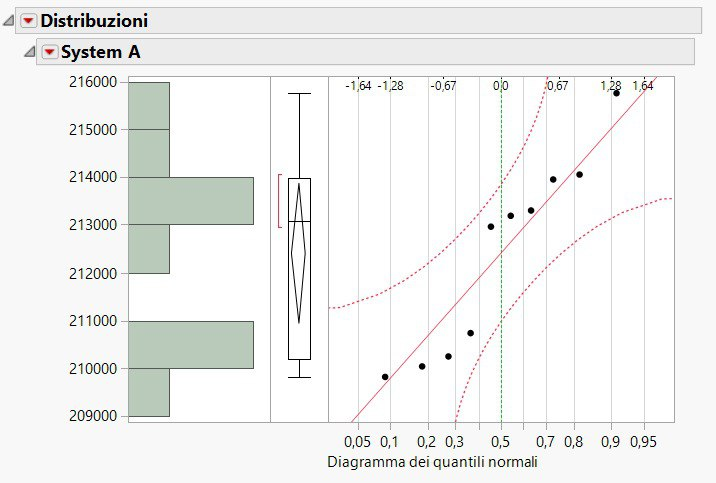
\includegraphics[width=\linewidth]{img/ch1/qqplot_a.png}
  \label{fig:qqplot_a}
\end{subfigure}%
\begin{subfigure}{.5\textwidth}
  \centering
  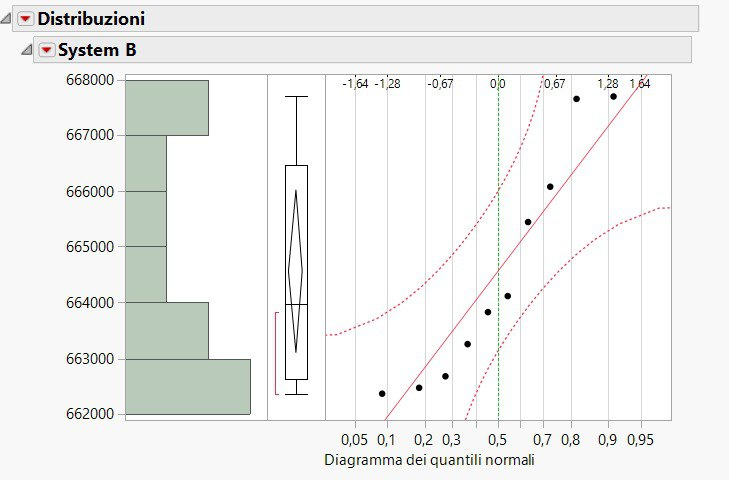
\includegraphics[width=\linewidth]{img/ch1/qqplot_b.png}
  \label{fig:qqplot_b}
\end{subfigure}
\caption{Plot quantile-quantile per Sistema A e Sistema B}
\label{fig:qqplot}
\end{figure}

Osservando i grafici in \cref{fig:qqplot}, si può concludere che entrambe le distribuzioni possono essere approssimate con una normale.

Sotto l'ipotesi di normalità, è possibile calcolare la \textit{sample size} usando la \cref{eq:sample_size}. 

\begin{equation}
    n = \left(\frac{z_{\alpha/2} \sigma}{E}\right)^2
    \label{eq:sample_size}
\end{equation}

In particolare, sfruttando i dati mostrati in \cref{table:10_samples}, scegliendo un intervallo di confidenza del $99\%$ e un errore pari a $0,01\%$ della media, è stato ottenuto il numero di campioni per entrambi i sistemi mostrati in \cref{tab:sample_size}.

\begin{table}[H]
\centering
    \begin{tabular}{|l|c|c|}
    \hline
    \multicolumn{1}{|c|}{\textbf{}} &
    \multicolumn{1}{c|}{\textbf{Sistema A}} & 
    \multicolumn{1}{c|}{\textbf{Sistema B}}  \tabularnewline \hline


Media & $644559.45$ & $212407.48$ \tabularnewline \hline
Dev.Std &$2047.23$ & $2051.20$
\tabularnewline \hline
\end{tabular}
\caption{Dati ottenuti prelevando in maniera preliminare $10$ campioni}
\label{table:10_samples}
\end{table}

\begin{table}[H]
\centering
    \begin{tabular}{|l|c|c|}
    \hline
    \multicolumn{1}{|c|}{\textbf{}} &
    \multicolumn{1}{c|}{\textbf{Sistema A}} & 
    \multicolumn{1}{c|}{\textbf{Sistema B}}  \tabularnewline \hline
    
Sample Size &$1.04$ & $10.27$ \tabularnewline \hline
\end{tabular}
\caption{Sample size ottenuta per entrambi i sistemi sotto l'ipotesi di normalità}
\label{tab:sample_size}
\end{table}

In base ai risultati ottenuti, si è deciso di procedere con $11$ campioni per entrambi i sistemi in modo da effettuare un \textit{paired test}.

\begin{table}[H]
\centering
    \begin{tabular}{|l|c|c|}
    \hline
    \multicolumn{1}{|c|}{\textbf{}} &
    \multicolumn{1}{c|}{\textbf{Sistema A}} & 
    \multicolumn{1}{c|}{\textbf{Sistema B}}  \tabularnewline \hline


Media & $644559.45$ & $212407.48$ \tabularnewline \hline
Dev.Std &$2047.23$ & $2051.20$ \tabularnewline \hline
\end{tabular}

\caption{Tabella riassuntiva dei due sistemi con $11$ campioni}
\end{table}

\section{Confronto tra i due sistemi}
Al fine di confrontare i due sistemi e verificare che le differenze tra le performance dei due sistemi sono statisticamente significative, si è scelto di operare un paired T-Test con $\alpha=0.05$ .

In \cref{fig:ris_ttest}, è mostrato il risultato del test, in cui appare chiaramente che tra i due sistemi c'è una differenza statistica.
\begin{figure}[H]
  \centering
  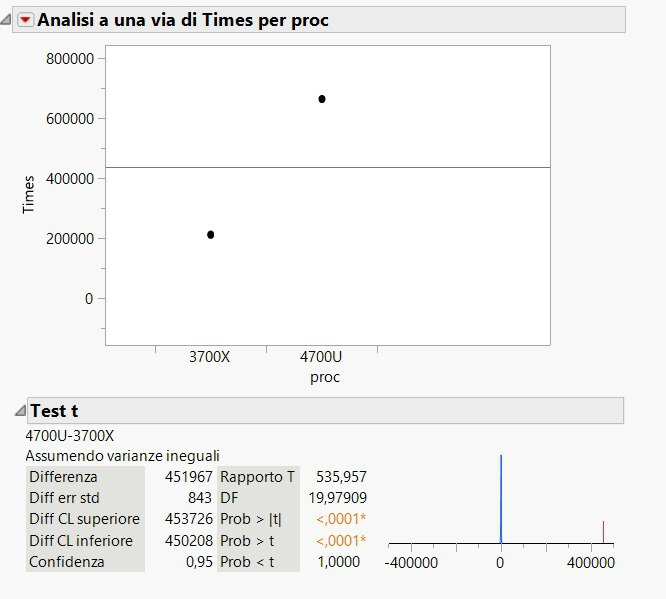
\includegraphics[width=\linewidth]{img/ch1/risultato_ttest.png}
  \caption{Risultati zero mean test con varianze ineguali}
  \label{fig:ris_ttest}
\end{figure}


